\chapter{Fundamentos de Elasticidade}\label{sec.fund_elast}

\section{Introdu\c{c}\~ao}
A teoria formal da propaga\c{c}\~ao de ondas s\'ismicas repousa nas intera\c{c}\~oes entre as particulas infinitesimais discretas do meio \`a medida que uma deforma\c{c}\~ao se propaga. \'E muito dif\'icil estudar individualmente cada uma dessas intera\c{c}\~oes, mas dados experimentais que foram coletados como resultados dessas intera\c{c}\~oes sugerem que as mesmas podem ser consideradas em conjunto. Assim, o estudo da propaga\c{c}\~ao de ondas s\'ismicas atrav\'es de camadas de subsuperf\'icie num material discretizado pode ser feito considerando o meio como cont\'inuo, e tais estudos s\~ao os objetos da \textit{mec\^anica do cont\'inuo}. 

No desenvolvimento te\'orico da mec\^anica do cont\'inuo nao s\~ao consideradas as caracter\'isticas at\^omicas da mat\'eria bem como as intera\c{c}\~oes entre essas part~\'iculas, ou seja, a mat\'eria n\~ao \'e estudada do ponto de vista microsc\'opico. Segundo \cite{slawinski}, tal abordagem se justifica pelo fato de que a mat\'eria \'e formada por part\'iculas suficientemente pouco espa\c{c}adas e suas caracter\'isticas e comportamento podem ser descritos por fun\c{c}\~oes cont\'inuas e diferenci\'aveis. Assim, \'e assummido que elementos infinitesimais da mat\'eria t\^em as mesmas propriedades observadas em experimentos macrosc\'opicos, pois essa hip\'otese permite a cria\c{c}\~ao de um modelo matem\'atico abstrato \textit{efetivo} na descri\c{c}\~ao da realidade f\'isica. Como exemplo, vamos considerar a cor de um objeto. Pr\'otons e el\'etrons n\~ao possuem cor, mas os meios materiais (que s\~ao formados por pr\'otons e el\'etrons) t\^em a capacidade de absorver ou refletir determinados comprimentos de ondas eletromagn\'eticas as quais determinam a cor de cada meio. Outros conceitos da mec\^anica do cont\'inuo sao elasticidade, viscosidade, fric\c{c}\~ao, rigidez, etc, como veremos mais a frente.


\section{Fatos experimentais}
A teoria sobre elasticidade est\'a baseada em conceitos primitivos e conclus\~oes estabelecidas a partir de fatos experimentais verificados em v\'arios textos sobre o assunto como \cite{liu}, \cite{dahlem} e \cite{slawinski}. Adicionalmente, em geral as equa\c{c}\~oes que governam a propaga\c{c}\~ao de ondas em meios el\'asticos s\~ao n\~ao-lineares. Contudo, em experimentos s\'ismicos foi constatado que aspectos importantes da propaga\c{c}\~ao de ondas podem ser analisados a partir de equa\c{c}\~oes lineares, resultando numa abordagem chamada \textit{teoria da elasticidade linearizada}.

\subsection{Deforma\c{c}\~ao}

A \textit{deforma\c{c}\~ao} de um meio el\'astico cont\'inuo \'e a mudan\c{c}a na posi\c{c}\~ao dos pontos que comp\~oem o corpo em rela\c{c}\~ao uns aos outros. Ou seja, h\'a uma mudan\c{c}a relativa entre os pontos e n\~ao um deslocamento do corpo como um todo e sem mudan\c{c}a de sua forma, caso em que ter\'iamos um \textit{movimento r\'igido}. Nesta subse\c{c}\~ao estamos interessados nas caracter\'isticas geom\'etricas relativas \`a deforma\c{c}\~ao de um corpo. N\~ao estamos considerando as causas de deforma\c{c}\~ao de um corpo, como aplica\c{c}\~ao de carga ou varia\c{c}\~ao de temperatura, nem discutiremos a composi\c{c}\~ao do material, assumindo apenas que o mesmo seja cont\'inuo e el\'astico. Assim, vamos relacionar as caracter\'isticas geom\'etricas de um corpo antes da deforma\c{c}\~ao com as caracter\'isticas ap\'os a deforma\c{c}\~ao.

\subsection{Dedu\c{c}\~ao do Tensor de Deforma\c{c}\~oes}\label{sec.deriva_deforma}

Para determinar o tensor de deforma\c{c}\~oes vamos considerar dois pontos pertencentes ao espaco $\mathbb{R}^3$ bastante pr\'oximos um do outro denotados por
\begin{align*}
\mathbf{x}&=(x_1,x_2,x_3)\quad\text{e}\\
\mathbf{y}=\mathbf{x}+d\mathbf{s}&=(x_1+dx_1,x_2+dx_2,x_3+dx_3),
\end{align*}
e que podem ser observados na figura \ref{fig.deformacao_meio}. O quadrado da dist\^ancia entre esses dois pontos \'e
\begin{equation}\label{eq.dist_antes_defor}
\norm{d\mathbf{s}}^2=(dx_1)^2+(dx_2)^2+(dx_3)^2.
\end{equation}
\begin{figure}
\centering
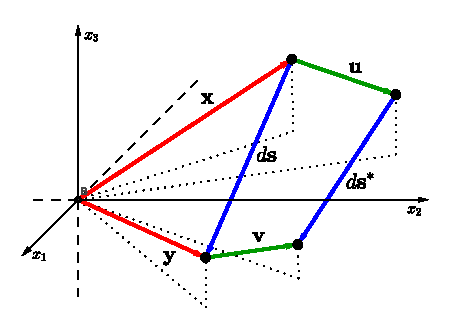
\includegraphics[scale=1.4]{deformacao_meio}
\caption{\textit{Mudan\c{c}a na posi\c{c}\~ao relativa entre os pontos que comp\~oem um  meio el\'astico cont\'inuo.}}
\label{fig.deformacao_meio}
\end{figure}
A aplica\c{c}\~ao de uma deforma\c{c}\~ao depende do ponto de aplica\c{c}\~ao, ou seja, a deforma\c{c}\~ao aplicada no ponto $\mathbf{x}$ difere da aplica\c{c}\~ao no ponto $\mathbf{y}$. Caso o vetor que d\'a a deforma\c{c}\~ao tenha componentes constantes, n\~ao teremos uma deforma\c{c}\~ao relativa, apenas uma transla\c{c}\~ao dos pontos. Assim, podemos definir o \textit{vetor de deslocamento} para cada ponto de aplica\c{c}\~ao
\begin{align*}
\mathbf{u}(\mathbf{x})&=(u_1,u_2,u_3),\\
\mathbf{v}(\mathbf{y})&=(v_1,v_2,v_3),
\end{align*}
e som\'a-los aos respectivos pontos $\mathbf{x}$ e $\mathbf{y}$ para obter suas posi\c{c}\~oes ap\'os a deforma\c{c}\~ao,
\begin{align*}
\mathbf{x}^*&=(x_1+u_1,x_2+u_2,x_3+u_3)\\
\mathbf{y}^*&=(x_1+dx_1+v_1,x_2+dx_2+v_2,x_3+dx_3+v_3).
\end{align*}
Subtraindo, obtemos o vetor que d\'a a diferen\c{c}a entre os pontos ap\'os a deforma\c{c}\~ao
\begin{equation}\label{eq.dist_apos_defor}
d\mathbf{s}^*=(dx_1+v_1-u_1,dx_2+v_2-u_2,dx_3+v_3-u_3).
\end{equation}
Como a varia\c{c}\~ao entre os pontos $\mathbf{x}$ e $\mathbf{y}$ \'e infinitesimal, vamos aplicar a expans\~ao de Taylor de segunda ordem em torno do ponto $\mathbf{x}$ e desprezar o resto de Lagrange para escrever as componentes de $\mathbf{v}$ em fun\c{c}\~ao das componentes de $\mathbf{u}$, aproximadamente,
\begin{align*}
v_1&\approx u_1+\frac{\partial u_1}{\partial x_1}\Bigg\vert_{\mathbf{x}}dx_1+\frac{\partial u_1}{\partial x_2}\Bigg\vert_{\mathbf{x}}dx_2+\frac{\partial u_1}{\partial x_3}\Bigg\vert_{\mathbf{x}}dx_3\\\\
v_2&\approx u_2+\frac{\partial u_2}{\partial x_1}\Bigg\vert_{\mathbf{x}}dx_1+\frac{\partial u_2}{\partial x_2}\Bigg\vert_{\mathbf{x}}dx_2+\frac{\partial u_2}{\partial x_3}\Bigg\vert_{\mathbf{x}}dx_3\\\\
v_3&\approx u_3+\frac{\partial u_3}{\partial x_1}\Bigg\vert_{\mathbf{x}}dx_1+\frac{\partial u_3}{\partial x_2}\Bigg\vert_{\mathbf{x}}dx_2+\frac{\partial u_3}{\partial x_3}\Bigg\vert_{\mathbf{x}}dx_3.
\end{align*}
Substituindo esses valores na equa\c{c}\~ao \ref{eq.dist_apos_defor}, simplificando e introduzindo a nota\c{c}\~ao de somat\'orio temos
\begin{equation*}
d\mathbf{s}^*\approx\left(dx_1+\sum_{i=1}^3\frac{\partial u_1}{\partial x_i}\Bigg\vert_{\mathbf{x}}dx_i\,,\,dx_2+\sum_{i=1}^3\frac{\partial u_2}{\partial x_i}\Bigg\vert_{\mathbf{x}}dx_i\,,\,dx_3+\sum_{i=1}^3\frac{\partial u_3}{\partial x_i}\Bigg\vert_{\mathbf{x}}dx_i\right).
\end{equation*}
O quadrado da dist\^ancia entre os pontos ap\'os a deforma\c{c}\~ao \'e dado por
\begin{equation*}
\norm{d\mathbf{s}^*}^2\approx\left(dx_1+\sum_{i=1}^3\frac{\partial u_1}{\partial x_i}\Bigg\vert_{\mathbf{x}}dx_i\right)^2+\left(dx_2+\sum_{i=1}^3\frac{\partial u_2}{\partial x_i}\Bigg\vert_{\mathbf{x}}dx_i\right)^2+\left(dx_3+\sum_{i=1}^3\frac{\partial u_3}{\partial x_i}\Bigg\vert_{\mathbf{x}}dx_i\right)^2.
\end{equation*}
Abrindo cada uma das parcelas quadr\'aticas, temos
\begin{align*}
\norm{d\mathbf{s}^*}^2&\approx(dx_1)^2+2\,dx_1\,\sum_{i=1}^3\frac{\partial u_1}{\partial x_i}\Bigg\vert_{\mathbf{x}}dx_i+\left(\sum_{i=1}^3\frac{\partial u_1}{\partial x_i}\Bigg\vert_{\mathbf{x}}dx_i\right)^2\\\\
&+(dx_2)^2+2\,dx_2\,\sum_{i=1}^3\frac{\partial u_2}{\partial x_i}\Bigg\vert_{\mathbf{x}}dx_i+\left(\sum_{i=1}^3\frac{\partial u_2}{\partial x_i}\Bigg\vert_{\mathbf{x}}dx_i\right)^2\\\\
&+(dx_3)^2+2\,dx_3\,\sum_{i=1}^3\frac{\partial u_3}{\partial x_i}\Bigg\vert_{\mathbf{x}}dx_i+\left(\sum_{i=1}^3\frac{\partial u_3}{\partial x_i}\Bigg\vert_{\mathbf{x}}dx_i\right)^2.
\end{align*}
Pela equa\c{c}\~ao \ref{eq.dist_antes_defor}, a coluna  da esquerda \'e $\norm{d\mathbf{s}}^2$. Como estamos trabalhando com quantidades infinitesimais, podemos negligenciar a coluna da direita por se tratar do quadrado do gradiente de cada componente do vetor de deslocamento num produto escalar com o vetor que d\'a a dist\^ancia entre os pontos $\mathbf{x}$  e $\mathbf{y}$. A coluna do meio se desdobra em dezoito parcelas que podem ser agrupadas novamente num somat\'orio duplo. Assim,
\begin{equation*}
\norm{d\mathbf{s}^*}^2\approx\norm{d\mathbf{s}}^2+\sum_{i=1}^3\sum_{j=1}^3\left(\frac{\partial u_i}{\partial x_j}\Bigg\vert_{\mathbf{x}}+\frac{\partial u_j}{\partial x_i}\Bigg\vert_{\mathbf{x}}\right)dx_i\,dx_j,
\end{equation*}
onde o termo entre par\^enteses \'e definido como o \textit{tensor de deforma\c{c}\~ao} na teoria da elasticidade,
\begin{equation*}
\varepsilon_{i,j}=\frac{1}{2}\left(\frac{\partial u_i}{\partial x_j}\Bigg\vert_{\mathbf{x}}+\frac{\partial u_j}{\partial x_i}\Bigg\vert_{\mathbf{x}}\right),\qquad\text{e}\qquad i,j\,\in\,\{1,2,3\}.
\end{equation*}
Considerando deslocamentos infinitesimais, os componentes desse tensor nos permitem descrever as deforma\c{c}\~oes associadas a esses deslocamentos entre os pontos iniciais. Analisando as entradas do tensor vemos que se o vetor de deslocamento \'e constante ent\~ao $\epsilon_{i,j}=0$ para todo o tensor, e n\~ao h\'a deforma\c{c}\~ao, apenas movimento r\'igido como descrito anteriormente. Como se trata de uma matriz sim\'etrica, no espa\c{c}o $\mathbb{R}^3$ temos apenas seis componentes independentes para o tensor.

\subsection{Interpreta\c{c}\~ao Geometrica do Tensor de Deforma\c{c}\~ao}

Existem basicamente dois tipos de deforma\c{c}\~oes descritas pelo tensor, uma onde podemos ter mudan\c{c}a de comprimento em alguma dimens\~ao ocasionando mudan\c{c}a de volume, mas sem mudan\c{c}a na forma do corpo estudado. Outra com mudan\c{c}a na forma mas sem mudan\c{c}a de volume. Vamos analisar como cada entrada do tensor \'e respons\'avel por altera\c{c}\~oes geom\'etricas do meio.

\subsubsection{Altera\c{c}\~ao Relativa de Comprimento}\label{sec.alte_compri}

Considerando o caso unidimensional, vamos aplicar as deforma\c{c}\~oes $\mathbf{u}$ e $\mathbf{v}$ aos pontos $\mathbf{x}=(x_1,0,0)$ e $\mathbf{y}=(x_1+dx_1,0,0)$, respectivamente,
\begin{equation*}
\mathbf{x}^*=(x_1+u_1,u_2,u_3)\quad\text{e}\quad\mathbf{y}^*=(x_1+dx_1+v_1,v_2,v_3).
\end{equation*}
Calculando a dist\^ancia entre os pontos ap\'os a deforma\c{c}\~ao temos
\begin{equation*}
d\mathbf{s}^*=(dx_1+v_1-u_1,v_2-u_2,v_3-u_3).
\end{equation*}
Analogamente a subse\c{c}\~ao \ref{sec.deriva_deforma}, vamos usar a expans\~ao de Taylor e ignorar o resto de Lagrange para escrever a primeira componente de $\mathbf{v}$ em fun\c{c}\~ao da primeira componente de $\mathbf{u}$. 
\begin{equation*}
v_1(\mathbf{y})=u_1(\mathbf{x})+\frac{\partial u_1}{\partial x_1}\Bigg\vert_{\mathbf{x}}dx_1+\frac{1}{2}\frac{\partial^2 u_1}{\partial x_1^2}\Bigg\vert_{\mathbf{x}}(dx_1)^2+\cdots
\end{equation*}
Novamente, utilizando a aproxima\c{c}\~ao para os dois primeiros termos e substituindo a primeira componente do vetor $d\mathbf{s}^*$, temos
\begin{equation}
dx_1^*\approx dx_1+\frac{\partial u_1}{\partial x_1}\Bigg\vert_{\mathbf{x}}dx_1\approx \left(1+\frac{\partial u_1}{\partial x_1}\Bigg\vert_{\mathbf{x}}\right)\,dx_1. 
\end{equation}
Usando a nota\c{c}\~ao dos componentes do tensor de deforma\c{c}\~ao, temos
\begin{equation}\label{eq.defor_unidi}
dx_1^*\approx(1+\epsilon_{11})\,dx_1.
\end{equation} 
Assim, vemos que $\epsilon_{11}$ \'e uma contra\c{c}\~ao ou dilata\c{c}\~ao ao longo do eixo $x_1$ e, analogamente, podemos demonstrar que $\epsilon_{22}$ e $\epsilon_{33}$ determinam a distens\~ao ou contra\c{c}\~ao ao longo dos eixos $x_2$ e $x_3$, respectivamente.
Utilizando um abuso de nota\c{c}\~ao, podemos escrever a express\~ao \ref{eq.defor_unidi} como
\begin{equation*}
\frac{dx_1^*}{dx\-1}\approx \frac{\partial x_1+\partial u_1}{\partial x_1},
\end{equation*}
e desse jeito podemos perceber que o fator $(1+\epsilon_{11})$ \'e uma mudan\c{c}a relativa (citada na subse\c{c}\~ao \ref{sec.deriva_deforma}) no comprimento ao longo do eixo $x_1$ devido a deforma\c{c}\~ao.

\subsubsection{Altera\c{c}\~ao Relativa de Volume}

Para estudar as altera\c{c}\~oes no volume de um s\'olido el\'astico vamos considerar uma caixa retangular (paralelep\'ipedo) com dimens\~oes $\Delta x_1, \Delta x_2\quad\text{e}\quad\Delta x_3$ nas dire\c{c}\~oes dos eixos coordenados.  Dessa forma, o volume do paralelep\'ipedo \'e dado por\begin{equation*}
V=\Delta x_1\,\Delta x_2\,\Delta x_3.
\end{equation*}
Conforme subse\c{c}\~ao \ref{sec.alte_compri}, aplicando a mudan\c{c}a relativa de comprimento a cada uma das tr\^es dimans\~oes, temos que ap\'os a deforma\c{c}\~ao, o volume do s\'olido \'e dado por
\begin{align}\nonumber
V^*&=(1+\epsilon_{11})\Delta x_1\,(1+\epsilon_{22})\Delta x_2\,(1+\epsilon_{33})\Delta x_3\\\label{eq.altera_volume}
&=(1+\epsilon_{11})\,(1+\epsilon_{22})\,(1+\epsilon_{33})\,V.
\end{align}
Como a deforma\c{c}\~ao aplicada tem tamanho infinitesimal, estamos supondo que as altera\c{c}\~oes relativas de comprimento n\~ao fujam significativamente das dire\c{c}\~oes can\^onicas dos eixos coordenados, assim h\'a altera\c{c}\~ao apenas no volume do s\'olido e n\~ao no seu formato. Ainda por conta do valores infinitesimais de $\epsilon_{ii}$, podemos negligenciar os termos n\~ao lineares resultantes da multiplica\c{c}\~ao na equa\c{c}\~ao \ref{eq.altera_volume} e aproximar o volume ap\'os a deforma\c{c}\~ao para
\begin{equation}\label{eq.altera_volume_2}
V^*\approx(1+\epsilon_{11}+\epsilon_{22}+\epsilon_{33})\,V.
\end{equation}
Observe que $\epsilon_{11}+\epsilon_{22}+\epsilon_{33}$ \'e o tra\c{c}o do tensor de deforma\c{c}\~ao, pode ser calculado atrav\'es do divergente do vetor de deslocamento e ser\'a denotado por $\varphi$ definindo a \textit{dilata\c{c}\~ao},
\begin{align*}
\varphi &=\epsilon_{11}+\epsilon_{22}+\epsilon_{33}\\
&=\frac{\partial u_1}{\partial x_1}+\frac{\partial u_2}{\partial x_2}+\frac{\partial u_3}{\partial x_3}\\
&=\left(\frac{\partial}{\partial x_1},\frac{\partial}{\partial x_2},\frac{\partial}{\partial x_3}\right)\cdot(u_1,u_2,u_3)\\
&=\nabla\cdot \mathbf{u}.
\end{align*}
Como o tra\c{c}o de uma matriz \'e um escalar e este n\~ao se altera quando \'e aplicada uma transforma\c{c}\~ao nos eixos coordenados, temos que a dilata\c{c}\~ao e a consequente altera\c{c}\~ao no volume de um s\'olido n\~ao depende do sistema de coordenadas escolhido. Manipulando a equa\c{c}\~ao \ref{eq.altera_volume_2} podemos constatar que a dilata\c{c}\~ao se trata de uma mudan\c{c}a relativa do volume
\begin{equation*}
\frac{V^*-V}{V}\approx\epsilon_{11}+\epsilon_{22}+\epsilon_{33}.
\end{equation*}

\subsubsection{Altera\c{c}\~ao Relativa na Forma}

O tensor de deforma\c{c}\~ao tamb\'em descreve uma mudan\c{c}a no formato do corpo, conforme podemos acompanhar pela figura \ref{fig.deforma_formato}, onde um rat\^angulo \'e transformado num paralelogramo. 
\begin{figure}
\centering
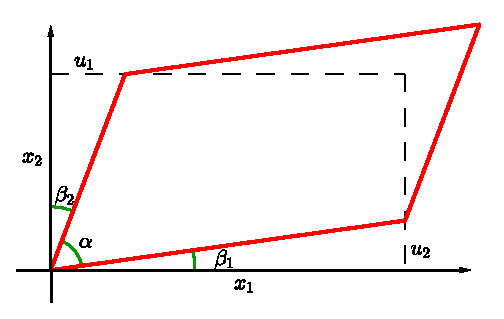
\includegraphics[scale=1.4]{deforma_formato}
\caption{\textit{Exemplo em duas dimens\~oes de como algumas componentes do tensor de deforma\c{c}\~ao promove a varia\c{c}\~ao no formato do meio.}}
\label{fig.deforma_formato}
\end{figure}
O angulo reto inicialmente formado pelos eixos coordenados $x_1$ e $x_2$ \'e reduzido a um \^angulo $\alpha$ que obedece \`a rela\c{c}\~ao
\begin{equation}
\alpha=\frac{\pi}{2}-\beta_1-\beta_2,
\end{equation}
onde $\beta_1$ e $\beta_2$ s\~ao os \^angulos formados pelos lados do paralelogramo e os eixos $x_1$ e $x_2$, respectivamente. Como a varia\c{c}\~ao angular \'e bastante pequena, temos que cada \^angulo $\beta_i$ pode ser aproximado por sua respectiva tangente, e considerando deslocamentos infinitesimais, temos
\begin{align*}
\beta_1+\beta_2&\approx\tan(\beta_1)+\tan(\beta_2)\\
&=\frac{\partial u_2}{\partial x_1}+\frac{\partial u_1}{\partial x_2}\\
&=2\epsilon_{12}=2\epsilon_{21}.
\end{align*}
Portanto, temos que o tensor de deforma\c{c}\~ao tamb\'em \'e respons\'avel pela altera\c{c}\~ao na dire\c{c}\~ao dos seguimentos que comp\~oem um corpo, mudando assim seu formato.


\subsection{Conserva\c{c}\~ao da Massa, Tens\~ao e o Equil\'ibrio do Momento Linear}

O princ\'ipio de conserva\c{c}\~ao da massa \'e fundamental em mec\^anica do cont\'inuo na determina\c{c}\~ao da rela\c{c}\~ao entre o vetor de deslocamento $\mathbf{u}$ e a densidade de massa de um corpo $\rho$. Por defini\c{c}\~ao, a quantidade de massa ocupando um volume $V$  num dado tempo $t$ \'e
\begin{equation}
m=\iiint_V\rho\,dV,
\end{equation}
onde tanto a massa como a densidade n\~ao dependem apenas do tempo mas tamb\'em da posi\c{c}\~ao $\mathbf{x}$. Fixado um volume $V$, a taxa de varia\c{c}\~ao da massa no tempo \'e dada por
\begin{equation}\label{eq.massa_1}
\frac{d}{dt}m=\iiint_V\frac{\partial\rho}{\partial t}dV.
\end{equation}
Assumindo que n\~ao h\'a destrui\c{c}\~ao nem produ\c{c}\~ao de massa dentro do volume, a varia\c{c}\~ao da massa se d\'a apenas pelo quantidade de massa que passa pelo volume, ou que passa atrav\'es de uma das superf\'icies que limita esse volume, o que pode ser escrito como
\begin{equation}\label{eq.massa_2}
\frac{dm}{dt}=-\iint_S\rho\,\mathbf{v}\cdot d\mathbf{S},
\end{equation}
onde $\mathbf{v}$ \'e a velocidade da quantidade de massa que atravessa a superf\'icie $S$. A superf\'icie infinitesimal $dS$ \'e pequena o suficiente para ser considerada plana e tem o mesmo fluxo de massa em todos os seus pontos, e o sinal negativo decorre do fato de que o vetor normal \`a superf\'icie aponta no sentido de sa\'ida do volume. 

Substituindo a equa\c{c}\~ao \ref{eq.massa_2} na equa\c{c}\~ao \ref{eq.massa_1} temos
\begin{equation}\label{eq.massa_3}
\iiint_V\frac{\partial\rho}{\partial t}dV=-\iint_S\rho\,\mathbf{v}\cdot d\mathbf{S},
\end{equation}
ou seja, a taxa de varia\c{c}\~ao da quantidade de massa num determinado volume \'e proporcional \`a taxa de varia\c{c}\~ao da quantidade de massa que atravessa a superf\'icie que limita esse volume. Pelo teorema do divergente temos que
\begin{equation}\label{eq.massa_divergente}
\iint_S\rho\,\mathbf{v}\cdot d\mathbf{S}=\iiint_V\nabla\cdot (\rho\,\mathbf{v})\,dV,
\end{equation}
onde substiutindo a equa\c{c}\~ao \ref{eq.massa_divergente} na equa\c{c}\~ao \ref{eq.massa_3} e agrupando os integrandos sob um mesmo volume, temos
\begin{equation}
\iiint_V\left[\frac{\partial\rho}{\partial t}+\nabla\cdot (\rho\,\mathbf{v})\right]\,dV=0,
\end{equation}
que \'e a equa\c{c}\~ao que descreve a \textit{conserva\c{c}\~ao de massa} num determinado volume $V$.



\section{Equações de Lamé}

\section{Generalizações da teoria}

\section{Conclusões}